\documentclass[a4paper,11pt]{report}
 
 \usepackage[left=3cm, right=3cm, top=3cm, bottom=3cm]{geometry}
\usepackage{graphicx}
\usepackage{listings}
\usepackage{titlesec}
\usepackage{fancyhdr}
\usepackage{epstopdf}
\usepackage{float}
\usepackage{amsmath}
\usepackage{setspace}
\usepackage{eufrak}
\usepackage{url}
\usepackage{xcolor}
\usepackage{courier}
 \newcommand{\textform}[1]{\fontsize{14}{20}\selectfont{#1}}
\pagestyle{fancy}
\fancyhf{}
\fancyhead[R]{\thepage}
\renewcommand{\chaptermark}[1]{\markboth{#1}{}}
\renewcommand{\headrulewidth}{1pt}
\renewcommand{\footrulewidth}{1pt}

\lhead{\footnotesize{BOLT MOCOBOT}}
\rhead{}
\lfoot{\footnotesize{Department of Mechanical \& Engg.}}
\cfoot{}
\rfoot{\thepage}

\titleformat{\chapter}[display]
{\normalfont\Large\bfseries\centering}{\chaptertitlename\
\thechapter}{20pt}{\Large}


%\title{\textbf{A seminar report on\\TRUSTWORTHINESS MANAGEMENT IN THE SOCIAL INTERNET OF THINGS} 
%}
%\author{\textbf{Deena Jose}}

\begin{document}

\thispagestyle{empty}
  \begin{center}
  \color{blue}
      \fontsize{22}{25}\selectfont{\textbf{GOVERNMENT POLYTECHNIC COLLEGE PERUMBAVOOR}}\\[.1cm]
            \fontsize{15}{25}\selectfont{\textbf{Koovappady P.O Ernakulam-683 544 Kerala
    }}\\[1.2cm]
\begin{figure}[h]
	\centering
	\hspace{21pt}
	
\includegraphics[width=.50\linewidth]{logo.png}
	\label{fig:logo.png}
\end{figure}
\color{red}
\fontsize{14}{25}\selectfont{\textbf{Semester - VI}}\\
\fontsize{14}{25}\selectfont{\textbf{Mechanical Engineering 2022-23}}\\[1.2cm]

\begin{center}
\color{brown}
\fontsize{14}{25}\selectfont{\textbf{SEMINAR REPORT}}\\[0.1cm]
\end{center}
\color{black}
    \fontsize{14}{25}\selectfont{on}\\[1cm]
    \fontsize{20}{25}\selectfont{\textbf{BOLT MOCOBOT}}\\[0.1cm]
    \fontsize{14}{25}\selectfont{\textbf{The Robo Cam}}\\[1.2cm]
    \fontsize{12}{25}\selectfont{\textbf{Submitted by}}\\[.2cm]
    \color{green}
    \fontsize{14}{25}\selectfont \bfseries{PETER STEVEN SIKKERA}\\[.1cm]
    \fontsize{12}{25}\selectfont{\textbf{20022099}}\\[.2cm]
\fontsize{12pt}{20}\selectfont
\thispagestyle{empty}
\end{center}


\newpage
  \thispagestyle{empty}

    \begin{center}
    \color{blue}
      \fontsize{14}{20}\selectfont \textbf{GOVERNMENT POLYTECHNIC COLLEGE PERUMBAVOOR}\\
     
    \fontsize{14}{20}\selectfont \textbf{
DEPARTMENT OF MECHANICAL ENGINEERING}\\[1.5cm]
\begin{figure}[h]
\centering
	\hspace{.5cm}

\includegraphics[width=0.3\linewidth]{logo.png}
	\label{fig:logo.png}
\end{figure}

     \color{red}
      \textbf{CERTIFICATE}
    \end{center}
    \vspace{.5cm}
    \textform{This is to certify that the seminar report entitled \textbf{Bolt Mocobot - The Robo Cam} submitted by \textbf{Peter Steven Sikkera},  is approved for submission requirement for Project and Seminar in  $6^{th}$ semester Mechanical Engineering at Govt.Polytechnic College,Perumbavoor.}\\[0.15cm]

        \begin{minipage}{.40\textwidth}
    \begin{flushleft}
        \begin{center}
            \fontsize{12}{25}\selectfont{\textbf{Head of Section}}\\[4cm]
        \end{center}
    \end{flushleft}
\end{minipage}
\hfill
\begin{minipage}{0.40\textwidth}
    \begin{flushright}
        \begin{center}
            \fontsize{12}{25}\selectfont{\textbf{Lecturer in Charge}}\\[4cm]
        \end{center}
    \end{flushright}
\end{minipage}




\vspace{1cm}
\begin{flushleft}
  \fontsize{12}{20}\selectfont \textbf{Date  :}\\
  \fontsize{12}{20}\selectfont \textbf{Place :}
\end{flushleft}

\vspace{1cm}
\begin{minipage}{.4\textwidth}
    \begin{flushleft}
    \begin{center}
    
    \fontsize{14}{25}\selectfont \bfseries{Internal Examiner}\\[.1cm]
    
%\vfill
 \end{center}
    \end{flushleft}
      \end{minipage}
\begin{minipage}{0.8\textwidth}
\begin{flushright}
\begin{center}
 
%\vfill
\fontsize{14}{25}\selectfont \bfseries{External Examiner}\\[.1cm]

\end{center}
\end{flushright}
\end{minipage}
\newpage
\fontsize{12pt}{20}\selectfont
\thispagestyle{empty}
  \renewcommand\abstractname{\textform{\textbf{ACKNOWLEDGMENT}}}
    \begin{abstract}
      \vspace{2.5cm}
    I would like to express my sincere gratitude to all those who have contributed to the successful completion of my seminar on Bolt Mocobot - The Robo Cam. This opportunity has allowed me to delve into a fascinating field of study and expand my knowledge in mechanical engineering.

First and foremost, I extend my heartfelt appreciation to Dr. Aiju Thomas, the Principal of Government Polytechnic College Perumbavoor. I am grateful for his constant support, guidance, and encouragement throughout my academic journey. His visionary leadership and commitment to excellence have created an environment conducive to learning and exploration.

I am indebted to Mr. Sivan P.K, the Head of the Department of Mechanical Engineering, for his invaluable guidance and mentorship. His expertise, patience, and enthusiasm have been instrumental in shaping my understanding of the subject and honing my research skills. I am thankful for his unwavering support and valuable insights that have enriched my seminar.

I would like to extend my sincere appreciation to the lecturers in Charge of Mechanical Engineering. His dedication to teaching and his willingness to go the extra mile in assisting students have been invaluable. I am grateful for his guidance, constructive feedback, and inspiring lectures that have helped me develop a deeper understanding of the topic.

I would like to express my gratitude to my classmates and friends for their support and encouragement. Their presence and collaboration have made the learning experience enjoyable and memorable.

Thank you all for your unwavering support and belief in me.
\begin{flushright}
  \fontsize{12}{20}\selectfont \textbf{PETER STEVEN SIKKERA}
\end{flushright}
    \end{abstract}
 


\thispagestyle{empty}
  \renewcommand\abstractname{\textform{\textbf{ABSTRACT}}}
    \begin{abstract}
      \vspace{1.0cm}

 \paragraph{ }High-speed cameras have revolutionized the world of cinematography, enabling filmmakers to capture stunning shots at frame rates exceeding 1,000 frames per second (fps). To further enhance the visual impact of these shots, filmmakers have sought ways to combine high-speed camera capabilities with fast camera movements. This demand for synchronized speed and motion has led to the development of the Bolt Mocobot.

The Bolt Mocobot is an innovative solution that not only delivers exceptional high-speed performance but also enables rapid camera movements. With the ability to reach full speed almost instantly, the Bolt Mocobot allows the camera to transition seamlessly from a standstill to high-speed motion and back in fractions of seconds. This unique capability empowers filmmakers to follow falling objects, capture dynamic action sequences, and create visually captivating scenes that were previously impossible to achieve by hand or other traditional methods.

By integrating state-of-the-art robotics technology, the Bolt Mocobot offers precise and automated control over camera movements. Filmmakers can program the Bolt Mocobot to execute complex and intricate camera motions with unrivaled precision, adding a new dimension to their storytelling. Whether it's tracking a moving subject, capturing fluid camera pans, or achieving seamless transitions between different shots, the Bolt Mocobot provides a level of speed and agility that enhances the creative possibilities of cinematography.

In this abstract, we explore the game-changing capabilities of the Bolt Mocobot. We delve into its ability to combine high-speed camera performance with rapid camera movements, enabling filmmakers to capture breathtaking visuals and immersive storytelling. We highlight how the Bolt Mocobot's instant acceleration and deceleration capabilities allow it to follow falling objects and seize fleeting moments with unparalleled precision. Furthermore, we discuss the integration of robotics technology, which provides filmmakers with automated and precise control over camera movements, revolutionizing the art of cinematography.
\end{abstract}

  \tableofcontents
\thispagestyle{empty}

\chapter{Introduction}

\paragraph{}
The world of commercials and films has been forever changed by the emergence of high-speed cameras, capable of capturing stunning shots at frame rates exceeding 1,000 frames per second (fps). These cameras have unlocked new dimensions of visual storytelling, allowing filmmakers to slow down time, capture intricate details, and create breathtaking visuals that captivate audiences. However, filmmakers have sought to push the boundaries further by combining high-speed camera capabilities with fast camera movements, resulting in the birth of the Bolt Mocobot.

The Bolt Mocobot represents a groundbreaking innovation that not only possesses exceptional high-speed performance but also enables rapid camera movements. Its ability to swiftly accelerate from a standstill to full speed and seamlessly transition back to a stationary position in a fraction of a second has revolutionized the way falling objects are captured, making shots that were once impossible now within reach. With the Bolt Mocobot, filmmakers can track and follow fast-moving subjects, capturing every fleeting moment with unprecedented precision, surpassing the limitations of manual operation or other conventional methods.

In this report, we delve into the extraordinary capabilities of the Bolt Mocobot, exploring its unique fusion of high-speed camera performance and rapid camera movements. We examine how its ability to swiftly reach full speed and decelerate with precision has revolutionized the capture of falling objects and the portrayal of fast-paced action. Furthermore, we explore the integration of robotics technology, providing filmmakers with a level of control and precision that transforms the art of cinematography.
  

  
\chapter{Technology Overview}
Bolt Mocobot - the RoboCam is an advanced high-speed camera technology that combines exceptional speed and precision with robotic control, revolutionizing the field of cinematography. This technology offers filmmakers the ability to capture stunning shots at incredibly high frame rates, often exceeding 1,000 frames per second (fps), while enabling dynamic camera movements with unparalleled accuracy.

The core component of Bolt Mocobot is the high-speed camera itself. It is designed to capture footage at ultra-fast frame rates, allowing filmmakers to slow down time and capture even the most fleeting moments in exquisite detail. The camera's impressive speed and frame rate capabilities make it ideal for capturing fast-paced action, sports sequences, and dynamic scenes.

What sets Bolt Mocobot apart is its integration of robotics technology, which adds a new dimension to camera movements. By incorporating robotic control systems, the camera can execute precise and complex movements, offering filmmakers a level of control that was previously challenging to achieve manually. This robotic control enables the camera to follow objects in motion, track subjects seamlessly, and capture shots from unique perspectives, enhancing the visual storytelling experience.

The robotic control system of Bolt Mocobot allows for highly accurate and repeatable camera movements. Filmmakers can program the camera to execute specific paths, angles, and trajectories, ensuring consistent and precise shots. This level of automation not only improves efficiency but also enables filmmakers to focus more on creativity and storytelling.

In terms of technical specifications, Bolt Mocobot is equipped with advanced sensors and image processing capabilities. These components work together to ensure exceptional image quality and clarity, even in challenging lighting conditions. The camera's high-resolution sensors capture detailed imagery, while advanced image processing algorithms enhance the final output, resulting in visually stunning footage.

Moreover, Bolt Mocobot offers seamless integration with existing production workflows. It can be synchronized with other camera systems, lighting setups, and post-production processes, allowing for seamless integration and compatibility within the filmmaking ecosystem.

Overall, Bolt Mocobot's technology represents a remarkable combination of high-speed camera capabilities and robotic control systems. This integration empowers filmmakers to capture breathtaking shots at incredibly high frame rates while executing precise and dynamic camera movements. The technology opens up new possibilities for creativity, allowing filmmakers to push the boundaries of visual storytelling and deliver immersive cinematic experiences.
\begin{figure}[h]
	\centering
	\hspace{21pt}
	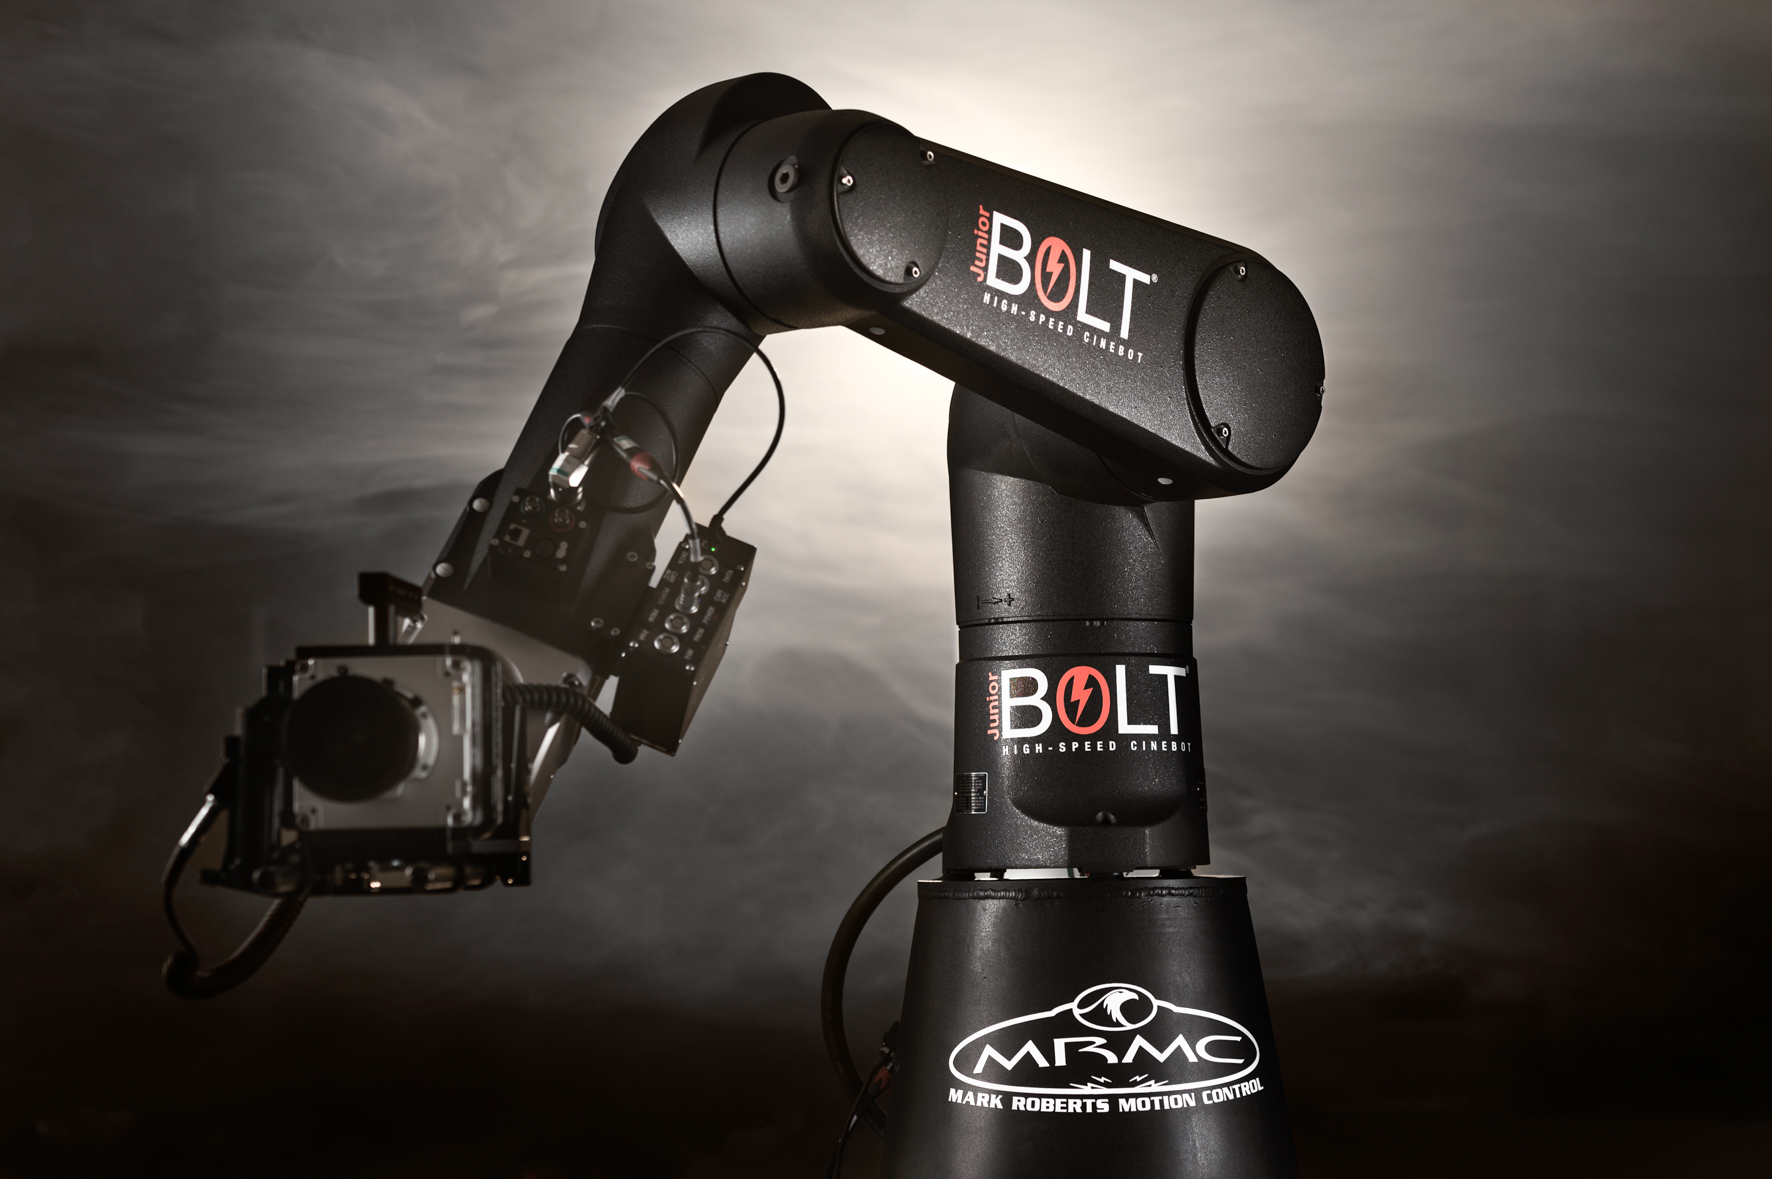
\includegraphics[width=.70\linewidth]{bolt.jpeg}
	\label{fig:logo.png}
\end{figure}

\chapter{Technical aspects}

\section{High-Speed Camera}
Bolt Mocobot incorporates a high-speed camera capable of capturing footage at frame rates exceeding 1,000 frames per second (fps) and even higher.
The camera utilizes advanced sensor technology to capture highly detailed imagery, ensuring exceptional image quality and clarity.
It offers a wide range of resolution options, allowing filmmakers to choose the appropriate level of detail for their specific requirements.
	
\section{Robotic Control System}
Bolt Mocobot integrates a sophisticated robotic control system that enables precise and automated camera movements.
The robotic control system can be programmed to execute complex camera paths, angles, and trajectories with remarkable accuracy.
It offers smooth and seamless movements, allowing for fluid camera pans, tracking shots, and dynamic camera movements.
\begin{figure}[h]
	\centering
	\hspace{21pt}
	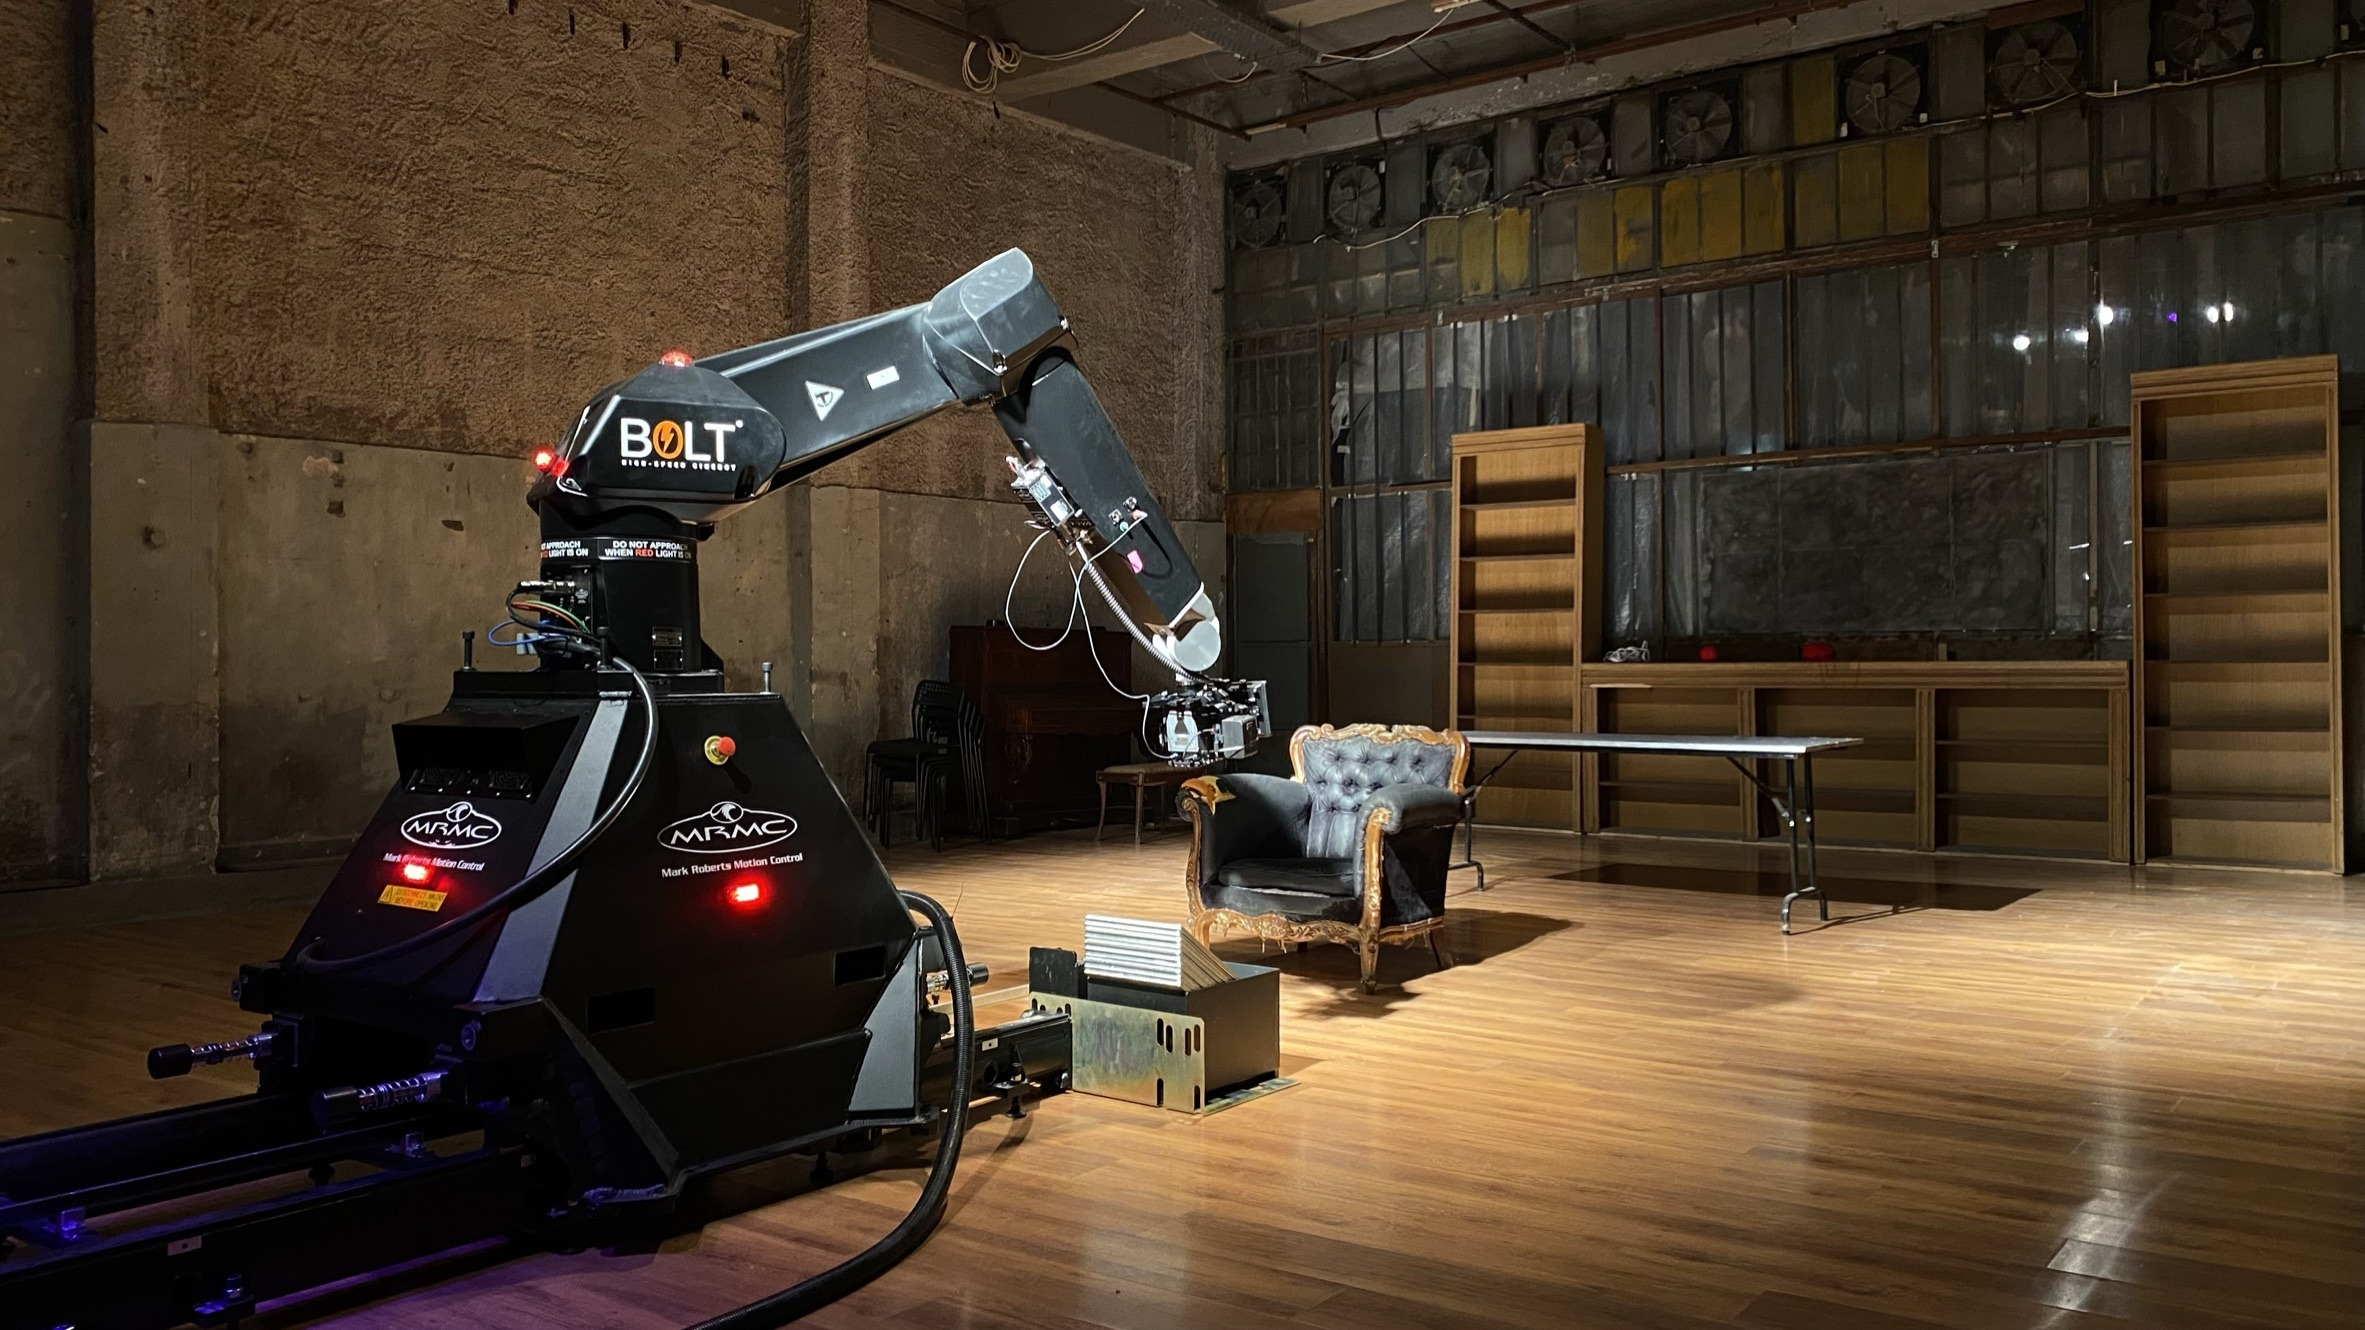
\includegraphics[width=.70\linewidth]{bolt1.jpeg}
	\label{fig:logo.png}
\end{figure}

\section{Rapid Acceleration and Deceleration}
One of the key technical features of Bolt Mocobot is its ability to reach full speed almost instantly and decelerate rapidly.
This rapid acceleration and deceleration enable the camera to capture shots with exceptional timing and precision, following fast-moving objects or subjects.

\section{Integration with Robotics Technology}
Bolt Mocobot seamlessly integrates with robotics technology, allowing for precise control over camera movements.
The camera can be controlled remotely using advanced control interfaces, enabling filmmakers to execute precise camera movements from a distance.
The integration of robotics technology ensures repeatability and consistency in camera movements, eliminating human error and variations.

\section{Ensemble Methods}
Ensemble methods combine multiple models to improve predictive performance. By leveraging the diversity and complementary strengths of individual models, ensemble techniques can achieve higher accuracy and reduce overfitting. Examples of ensemble methods include bagging (bootstrap aggregating), boosting (e.g., AdaBoost, Gradient Boosting), and random forests.

\section{Sensor and Image Processing}
Bolt Mocobot utilizes high-resolution sensors to capture detailed imagery with excellent dynamic range and low noise levels.
The camera's advanced image processing algorithms enhance the captured footage, improving image quality and optimizing color accuracy.
The combination of high-quality sensors and advanced image processing contributes to the production of visually stunning and impactful visuals.

\chapter{Challenges and Limitations}
While Bolt Mocobot - the RoboCam offers remarkable capabilities in high-speed cinematography, there are some challenges and limitations to consider. These include:

\section{Setup Complexity}
Setting up and configuring Bolt Mocobot can be a complex process. The integration of robotics technology requires technical expertise and specialized knowledge. Calibration and synchronization with other equipment, such as lighting setups or camera rigs, may also require additional time and resources.

\section{Space and Mobility}
Bolt Mocobot, being a sophisticated camera system, may require a dedicated space or rigging for optimal operation. The equipment itself can be bulky and may limit its mobility in certain shooting environments. Filmmakers need to consider the available space and assess whether the system can be deployed effectively in different shooting scenarios.

\section{Environmental Constraints}
Bolt Mocobot's performance may be affected by environmental factors such as temperature, humidity, and vibrations. Extreme conditions or uncontrolled environments may impact the camera's functionality and the quality of the footage. Filmmakers should take precautions and consider environmental factors when planning shoots.

\section{Post-Production Processing}
The high-speed footage captured by Bolt Mocobot requires extensive post-production processing and storage capacity. The large volume of data generated by high frame rates demands powerful computing resources and efficient data management. Post-production workflows need to accommodate the requirements for processing, editing, and storing high-speed footage effectively.

\chapter{Advantages}

\section{Rapid Camera Movements}
One of the key advantages of Bolt Mocobot is its ability to execute rapid camera movements with precision. The integration of robotics technology enables the camera to follow objects in motion seamlessly, providing dynamic and engaging shots that enhance visual storytelling.

\section{Instant Acceleration and Deceleration}
Bolt Mocobot can reach full speed almost instantly and decelerate rapidly. This allows filmmakers to capture shots with impeccable timing, following falling objects or fast-moving subjects. The ability to quickly transition between standstill and high-speed motion opens up new creative possibilities.

\section{Integration with Existing Workflows}
Bolt Mocobot seamlessly integrates with existing production workflows, making it compatible with other camera systems, lighting setups, and post-production processes. This allows for a smooth and efficient integration into the filmmaking process without major disruptions or additional complexities.

\section{Versatility in Applications}
Bolt Mocobot finds applications across various industries, including commercials, films, documentaries, sports, and scientific research. Its high-speed capabilities and dynamic camera movements make it suitable for capturing fast-paced action, analyzing motion, and revealing intricate details.

\chapter{Applications}
\section{Engineering and Manufacturing}
Bolt Mocobot is utilized in engineering and manufacturing industries for motion analysis, quality control, and process optimization. It can capture high-speed events on production lines, analyze machinery movements, and identify potential issues or areas for improvement. The camera's precise movements and ability to follow fast-paced actions aid in monitoring and enhancing manufacturing processes.
\section{Commercials and Advertising}
Bolt Mocobot is widely utilized in the creation of commercials and advertising campaigns. Its high-speed capabilities enable the capture of fast-paced product shots, emphasizing details and creating visually stunning imagery. The camera's dynamic movements add a captivating element to the visuals, making the commercials more engaging and memorable.
\section{Scientific Research and Analysis}
Bolt Mocobot plays a crucial role in scientific research and analysis, particularly in fields that require detailed motion analysis. It can capture high-speed events and movements with exceptional accuracy, allowing researchers to study and analyze intricate motions in various disciplines such as biomechanics, robotics, sports science, and more.
\section{Slow-Motion Cinematography}
Bolt Mocobot is renowned for its ability to capture breathtaking slow-motion footage. This makes it a valuable tool for cinematographers and filmmakers who want to emphasize specific moments or create dramatic effects. The camera's high frame rates and precise movements enable the creation of visually striking slow-motion sequences.
\section{Automotive Industry}
Bolt Mocobot has applications in the automotive industry, particularly in the development and testing of vehicles. It can capture high-speed events during crash tests, performance analysis, and aerodynamics research. The camera's ability to follow fast-moving objects and execute precise movements aids in analyzing vehicle behavior and safety measures.

\chapter{Conclusion}
In conclusion, Bolt Mocobot represents a groundbreaking innovation in the field of cinematography and high-speed camera technology. With its ability to capture footage at frame rates exceeding 1,000 frames per second (fps) and execute rapid camera movements, Bolt Mocobot opens up new possibilities for filmmakers and professionals across various industries.

The integration of advanced robotics technology allows Bolt Mocobot to achieve instant acceleration and deceleration, enabling the camera to follow fast-moving objects and capture shots with exceptional timing and precision. This not only enhances the visual aesthetics of films, commercials, and television productions but also finds applications in scientific research, sports analysis, manufacturing, and other fields that require detailed motion analysis.

As technology continues to evolve, Bolt Mocobot represents a significant advancement in the realm of high-speed cameras, paving the way for new possibilities in visual storytelling, analysis, and creative expression. Its ability to capture fast-paced action, intricate details, and unique perspectives contributes to the creation of impactful cinematic experiences that captivate and engage audiences.

In summary, Bolt Mocobot revolutionizes the way filmmakers capture high-speed action, enabling them to push the boundaries of visual storytelling and deliver exceptional content across various industries. Its technical capabilities, versatility, and integration potential make it a valuable asset for professionals seeking to achieve stunning visuals, precise motion analysis, and immersive storytelling.

\chapter{References}

\begin{itemize}
\item[[1]] Stable visual servoing of camera-in-hand robotic systems

https://ieeexplore.ieee.org/abstract/document/828588

\item[[2]] A generic fisheye camera model for robotic applications

https://ieeexplore.ieee.org/abstract/document/4399233

\item[[3]] Designing Robotic Camera Systems to Enable Synchronous Remote Collaboration

https://dl.acm.org/doi/abs/10.1145/3568294.3579974

\item[[4]] Efficiency in image-guided robotic and conventional camera steering: a prospective randomized controlled trial

https://link.springer.com/article/10.1007/s00464-021-08508-9

\vspace{12pt}
\end{itemize}
\end{document}
